\documentclass[journal,12pt,twocolumn]{IEEEtran}
%
\usepackage{setspace}
\usepackage{gensymb}
\singlespacing
\usepackage[cmex10]{amsmath}
\usepackage{siunitx}
\usepackage{amsthm}

\usepackage{mathrsfs}

\usepackage{txfonts}
\usepackage{stfloats}

\usepackage{steinmetz}
\usepackage{cite}
\usepackage{cases}
\usepackage{subfig}
\usepackage{longtable}
\usepackage{multirow}
\usepackage{enumitem}
\usepackage{mathtools}
\usepackage{tikz}
\usepackage{circuitikz}
\usepackage{verbatim}
\usepackage{tfrupee}
\usepackage[breaklinks=true]{hyperref}
\usepackage{tkz-euclide} % loads  TikZ and tkz-base
\usetikzlibrary{calc,math}
\usetikzlibrary{fadings}
\usepackage{listings}
    \usepackage{color}                                            %%
    \usepackage{array}                                            %%
    \usepackage{longtable}                                        %%
    \usepackage{calc}                                             %%
    \usepackage{multirow}                                         %%
    \usepackage{hhline}                                           %%
    \usepackage{ifthen}                                           %%
  %optionally (for landscape tables embedded in another document): %%
    \usepackage{lscape}     
\usepackage{multicol}
\usepackage{chngcntr}
\DeclareMathOperator*{\Res}{Res}

\renewcommand\thesection{\arabic{section}}
\renewcommand\thesubsection{\thesection.\arabic{subsection}}
\renewcommand\thesubsubsection{\thesubsection.\arabic{subsubsection}}

\renewcommand\thesectiondis{\arabic{section}}
\renewcommand\thesubsectiondis{\thesectiondis.\arabic{subsection}}
\renewcommand\thesubsubsectiondis{\thesubsectiondis.\arabic{subsubsection}}

\hyphenation{op-tical net-works semi-conduc-tor}
\def\inputGnumericTable{}                                 %%

\lstset{
%language=C,
frame=single, 
breaklines=true,
columns=fullflexible
}
\begin{document}
%


\newtheorem{theorem}{Theorem}[section]
\newtheorem{problem}{Problem}
\newtheorem{proposition}{Proposition}[section]
\newtheorem{lemma}{Lemma}[section]
\newtheorem{corollary}[theorem]{Corollary}
\newtheorem{example}{Example}[section]
\newtheorem{definition}[problem]{Definition}
\newcommand{\BEQA}{\begin{eqnarray}}
\newcommand{\EEQA}{\end{eqnarray}}
\newcommand{\define}{\stackrel{\triangle}{=}}
\bibliographystyle{IEEEtran}
\providecommand{\mbf}{\mathbf}
\providecommand{\pr}[1]{\ensuremath{\Pr\left(#1\right)}}
\providecommand{\qfunc}[1]{\ensuremath{Q\left(#1\right)}}
\providecommand{\sbrak}[1]{\ensuremath{{}\left[#1\right]}}
\providecommand{\lsbrak}[1]{\ensuremath{{}\left[#1\right.}}
\providecommand{\rsbrak}[1]{\ensuremath{{}\left.#1\right]}}
\providecommand{\brak}[1]{\ensuremath{\left(#1\right)}}
\providecommand{\lbrak}[1]{\ensuremath{\left(#1\right.}}
\providecommand{\rbrak}[1]{\ensuremath{\left.#1\right)}}
\providecommand{\cbrak}[1]{\ensuremath{\left\{#1\right\}}}
\providecommand{\lcbrak}[1]{\ensuremath{\left\{#1\right.}}
\providecommand{\rcbrak}[1]{\ensuremath{\left.#1\right\}}}
\theoremstyle{remark}
\newtheorem{rem}{Remark}
\newcommand{\sgn}{\mathop{\mathrm{sgn}}}
\providecommand{\abs}[1]{\left\vert#1\right\vert}
\providecommand{\abs}[1]{\lvert#1\rvert} 
\providecommand{\res}[1]{\Res\displaylimits_{#1}} 
\providecommand{\norm}[1]{\left\lVert#1\right\rVert}
%\providecommand{\norm}[1]{\lVert#1\rVert}
\providecommand{\mtx}[1]{\mathbf{#1}}
\providecommand{\mean}[1]{E\left[ #1 \right]}
\providecommand{\fourier}{\overset{\mathcal{F}}{ \rightleftharpoons}}
%\providecommand{\hilbert}{\overset{\mathcal{H}}{ \rightleftharpoons}}
\providecommand{\system}{\overset{\mathcal{H}}{ \longleftrightarrow}}
	%\newcommand{\solution}[2]{\textbf{Solution:}{#1}}
\newcommand{\solution}{\noindent \textbf{Solution: }}
\newcommand{\cosec}{\,\text{cosec}\,}
\providecommand{\dec}[2]{\ensuremath{\overset{#1}{\underset{#2}{\gtrless}}}}
\newcommand{\myvec}[1]{\ensuremath{\begin{pmatrix}#1\end{pmatrix}}}
\newcommand{\mydet}[1]{\ensuremath{\begin{vmatrix}#1\end{vmatrix}}}
\numberwithin{equation}{subsection}
\makeatletter
\@addtoreset{figure}{problem}
\makeatother
\let\StandardTheFigure\thefigure
\let\vec\mathbf
\renewcommand{\thefigure}{\theproblem}
\def\putbox#1#2#3{\makebox[0in][l]{\makebox[#1][l]{}\raisebox{\baselineskip}[0in][0in]{\raisebox{#2}[0in][0in]{#3}}}}
     \def\rightbox#1{\makebox[0in][r]{#1}}
     \def\centbox#1{\makebox[0in]{#1}}
     \def\topbox#1{\raisebox{-\baselineskip}[0in][0in]{#1}}
     \def\midbox#1{\raisebox{-0.5\baselineskip}[0in][0in]{#1}}
\vspace{3cm}
\title{ASSIGNMENT-2}
\author{T.Naveena}
\maketitle
\newpage
\bigskip
\renewcommand{\thefigure}{\theenumi}
\renewcommand{\thetable}{\theenumi}
Download all python codes from 
\begin{lstlisting}
https://github.com/ThurpuNaveena/ASSIGNMENT-2/tree/main/CODES
\end{lstlisting}
%
and latex-tikz codes from 
%
\begin{lstlisting}
https://github.com/ThurpuNaveena/ASSIGNMENT-2/tree/main
\end{lstlisting}
%
\section{QUESTION NO-2.14 (linear forms)} Find the equation of the line satisfying the following conditions
\begin{enumerate}
\item Intersecting the x-axis at a distance of 3 units to the let of the origin with slope -2.
\item Intersecting the y-axis at a distance of 2 units above the origin and making an angle of $30\degree$ with the positive direction of the x-axis.
\end{enumerate}
%

%
\section{Solution}
\begin{enumerate}
\item Let line $AB$ intersect the x-axis at a distance 3 units to the  let of origin.
At x-axis, y is always 0.
slope $m = -2$.
The direction vector is $\vec{m} = \myvec{1\\-2}$.  
Hence, the normal vector
\begin{align}
\label{eq:line_norm_dir}
\vec{n} &= \myvec{0&-1\\1&0}\vec{m} 
\\
&= \myvec{2\\1}
\end{align}
The equation of the line in terms of the normal vector is then obtained as
\begin{align}
\label{eq:line_norm_vec}
\vec{n}^T\brak{\vec{x}-\vec{A}} &= 0
\\
\implies \myvec{2 & 1} \vec{x} &= -6
\end{align}
\begin{align}
\vec{A} = \myvec{-3\\0}, \vec{B} = \myvec{0\\-6}
\end{align}
Plot of the line $AB$
\numberwithin{figure}{section}
\begin{figure}[ht]
\centering
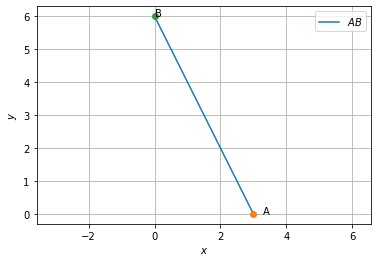
\includegraphics[width=\columnwidth]{Line_Plot_Part-1.PNG}
\caption{Plot of Line $AB$ (Part-1)}
\label{Plot of Line $AB$ (Part-1)}
\end{figure}
\item Line $AB$ intersects the y-axis 2 units above origin.
As we know that at y-axis,x-coordinate will be 0 always.
From the given information we have, $\tan30\degree =m = \frac{1}{\sqrt{3}}$.
\end{enumerate}
The direction vector is $\vec{m} = \myvec{1\\\tan30\degree}$.  
Hence, the normal vector
\begin{align}
\label{eq:line_norm_dir}
\vec{n} &= \myvec{0&-1\\1&0}\vec{m} 
\\
&= \myvec{-\tan30\degree\\1}
\end{align}
The equation of the line in terms of the normal vector is then obtained as
\begin{align}
\label{eq:line_norm_vec}
\vec{n}^T\brak{\vec{x}-\vec{A}} &= 0
\\
\implies \myvec{-1 &\sqrt{3}}\vec{x} &=2{\sqrt{3}}
\end{align}
\begin{align}
\vec{A} = \myvec{-2\sqrt{3}\\0},\vec{B} = \myvec{0\\2}
\end{align}
Plot of the line $AB$ 
\numberwithin{figure}{section}
\begin{figure}[ht]
\centering
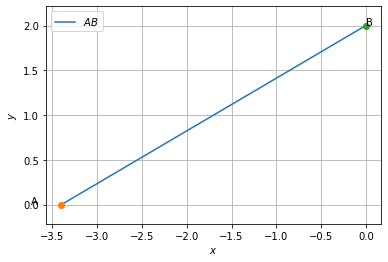
\includegraphics[width=\columnwidth]{Line_Plot_Part-2.PNG}
\caption{Plot of Line $AB$ (Part-2)}
\label{Plot of Line $AB$ (Part-2)}
\end{figure}
\end{document}
